% !TEX root = ../supp.tex
\begin{figure}
\centering
% \vspace{-0.1in}
\iflatexml
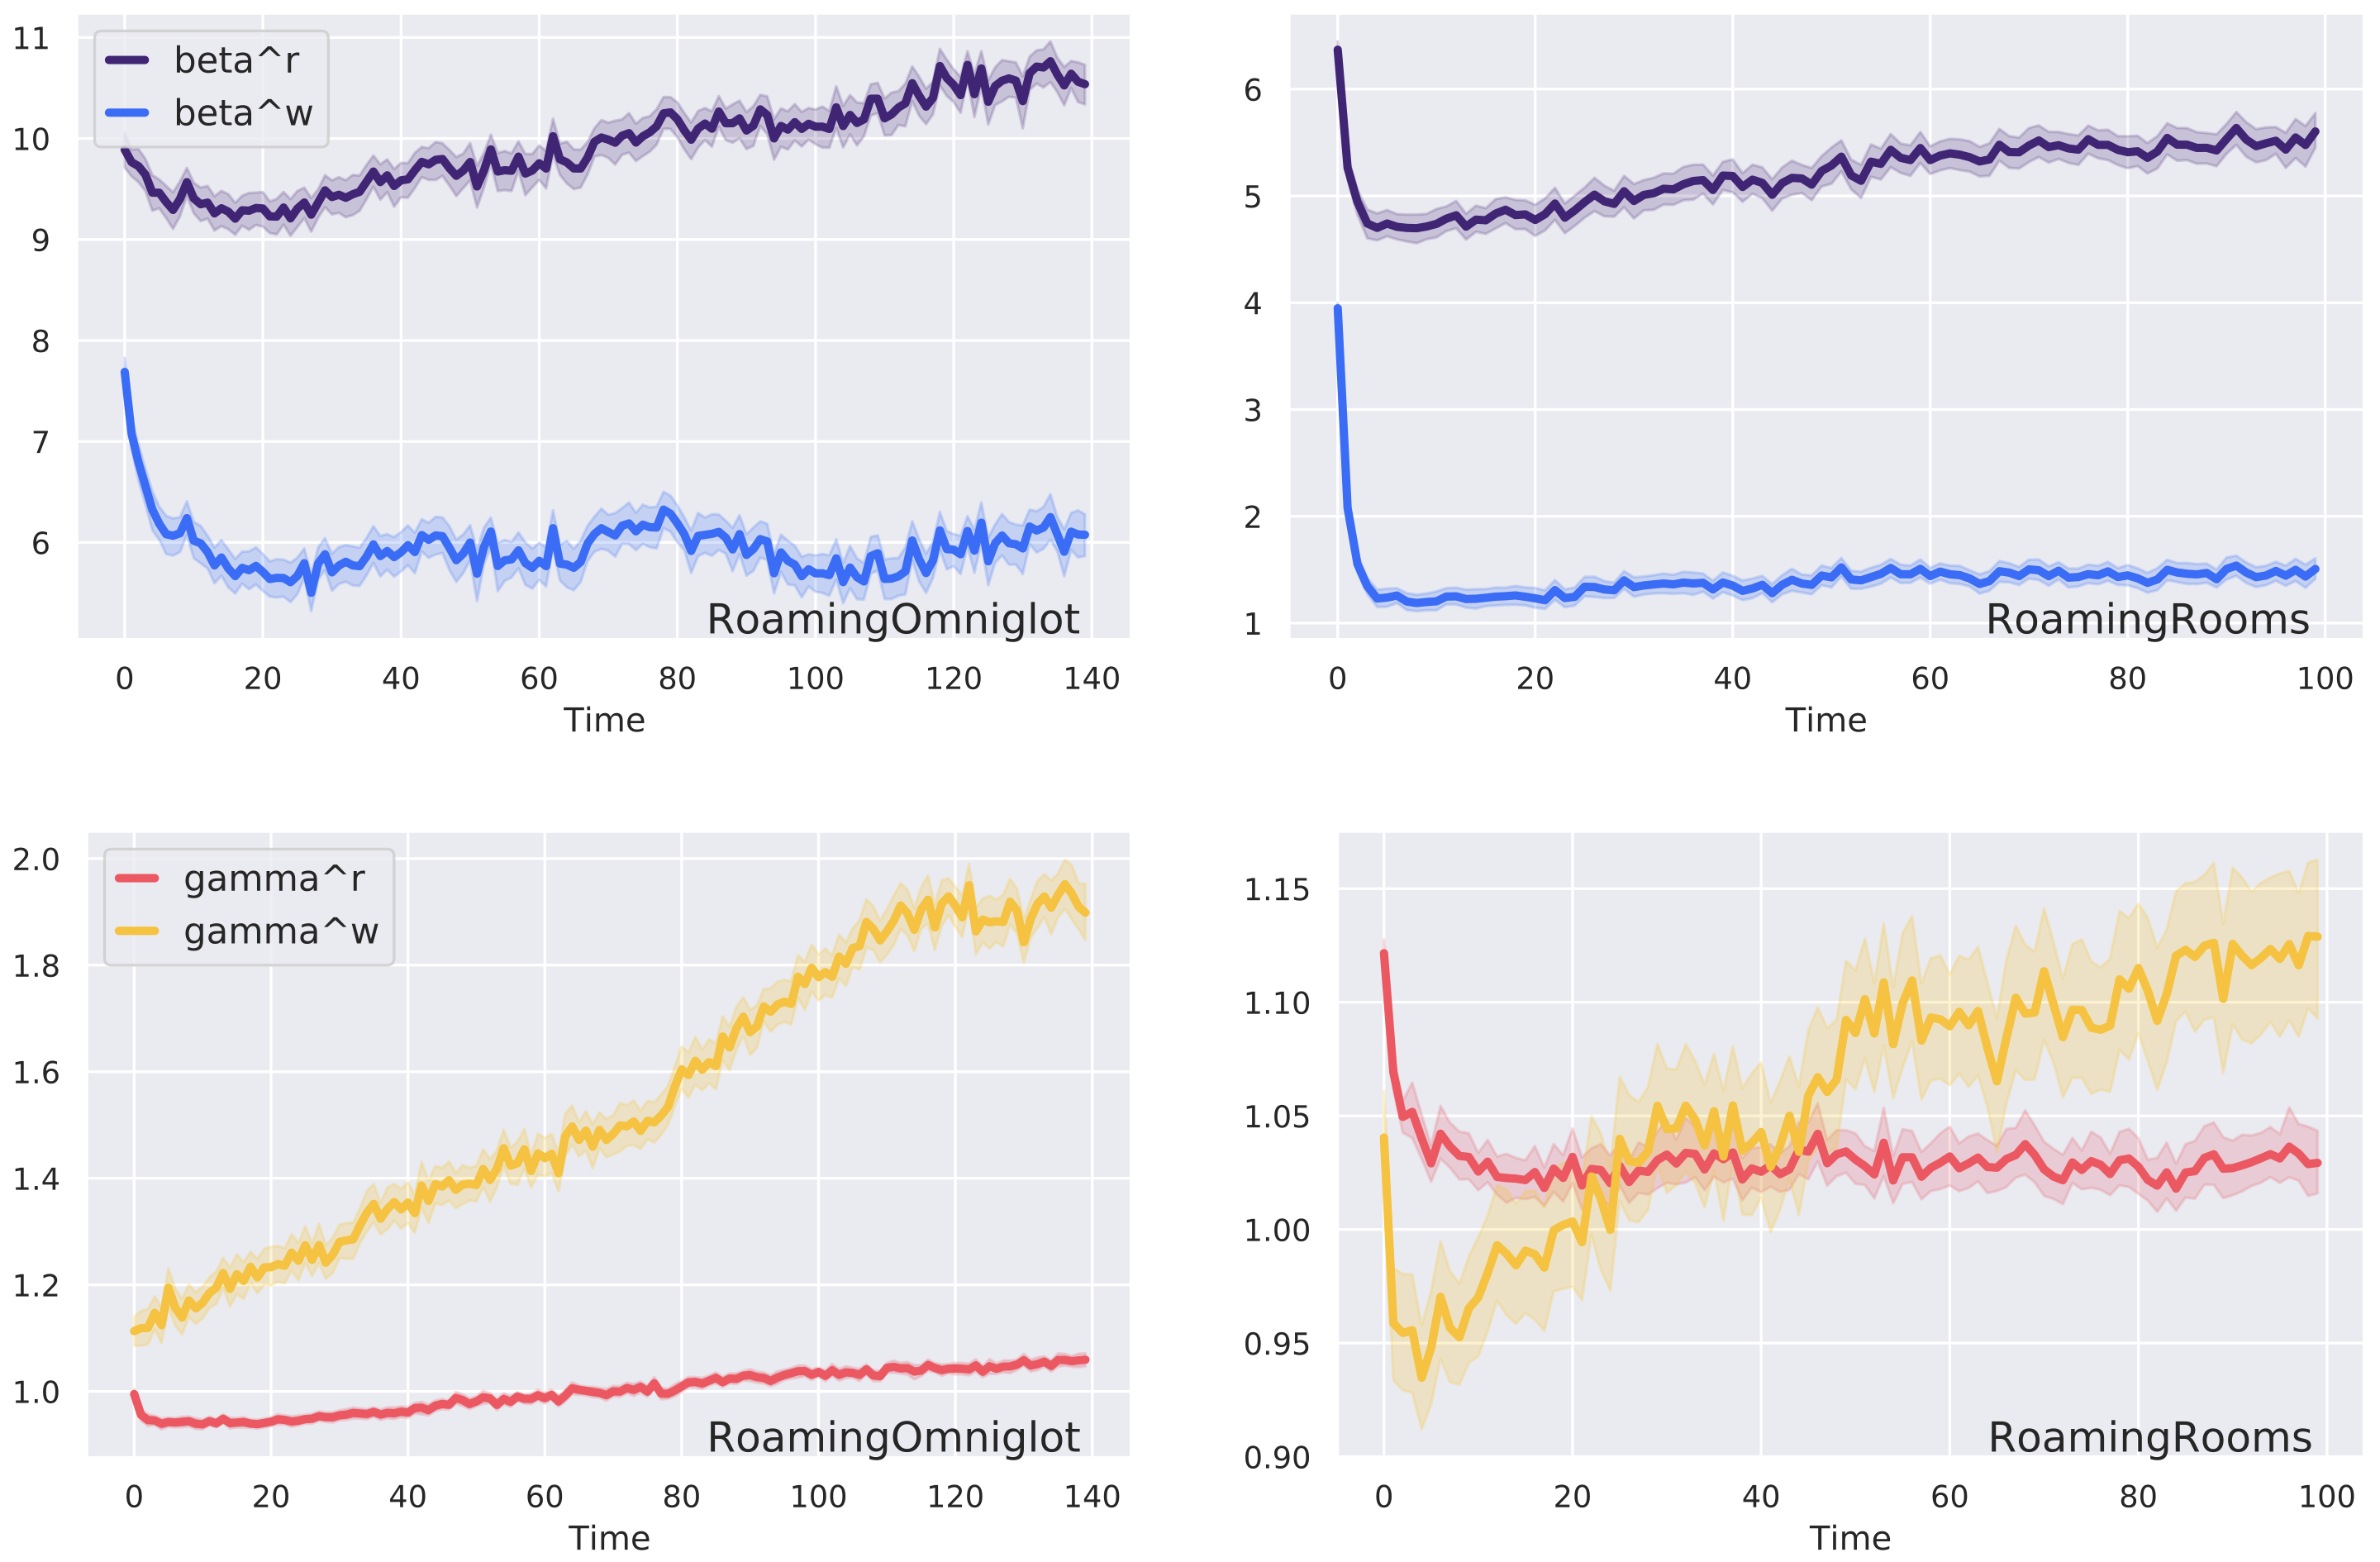
\includegraphics[width=6\linewidth]{figures/beta-gamma.png}
\else
\begin{tabular}{cc}
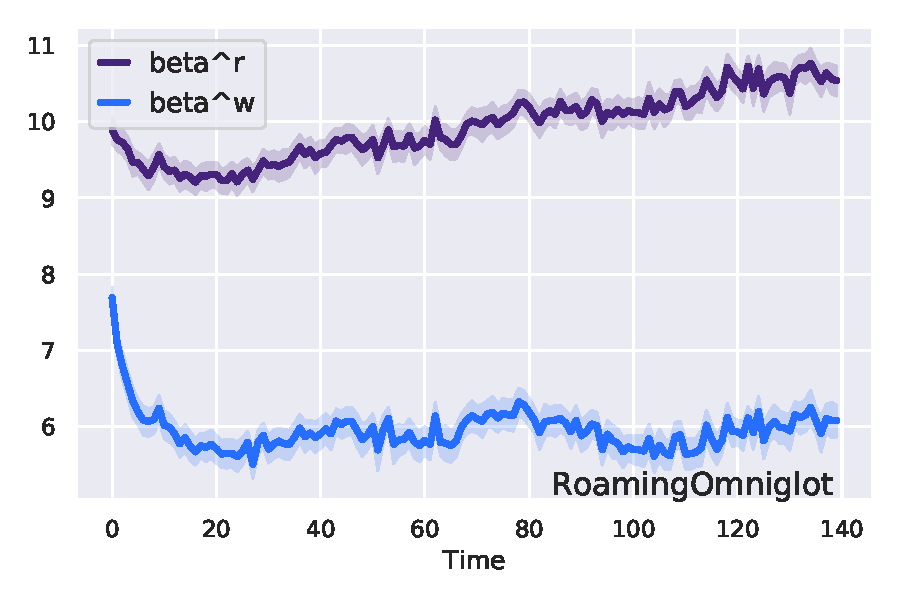
\includegraphics[height=4.0cm,trim={0.3cm 0cm 0.5cm 0},clip]{figures/omniglot-beta.pdf}
\quad
&
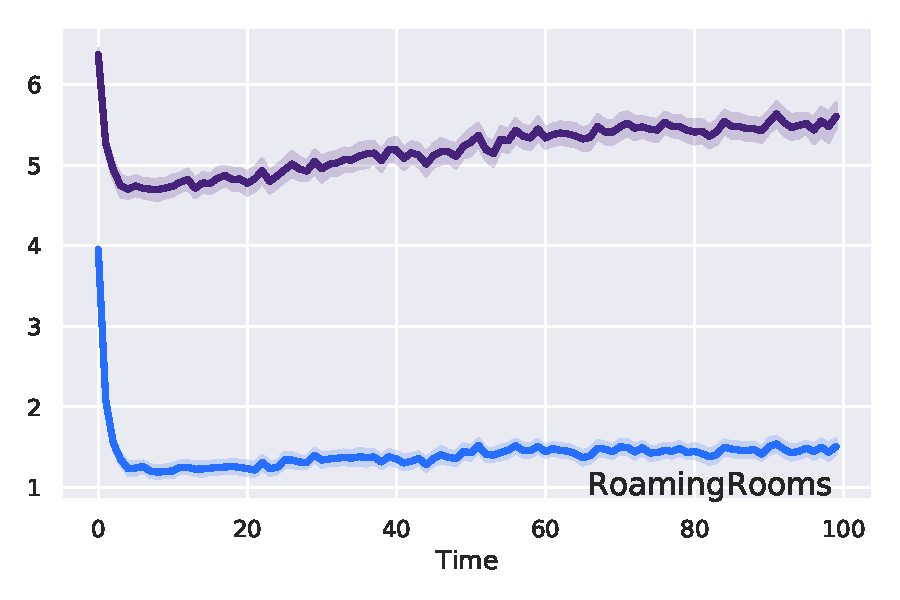
\includegraphics[height=4.0cm,trim={0.3cm 0cm 0cm 0},clip]{figures/matterport-beta.pdf}
\\
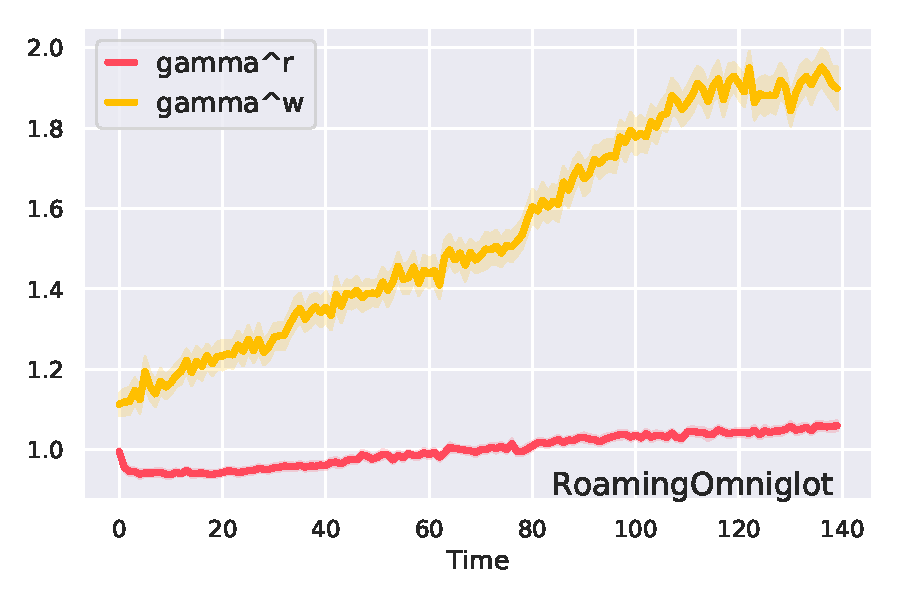
\includegraphics[height=4.0cm,trim={0.3cm 0cm 0.5cm 0},clip]{figures/omniglot-gamma.pdf}
\quad
&
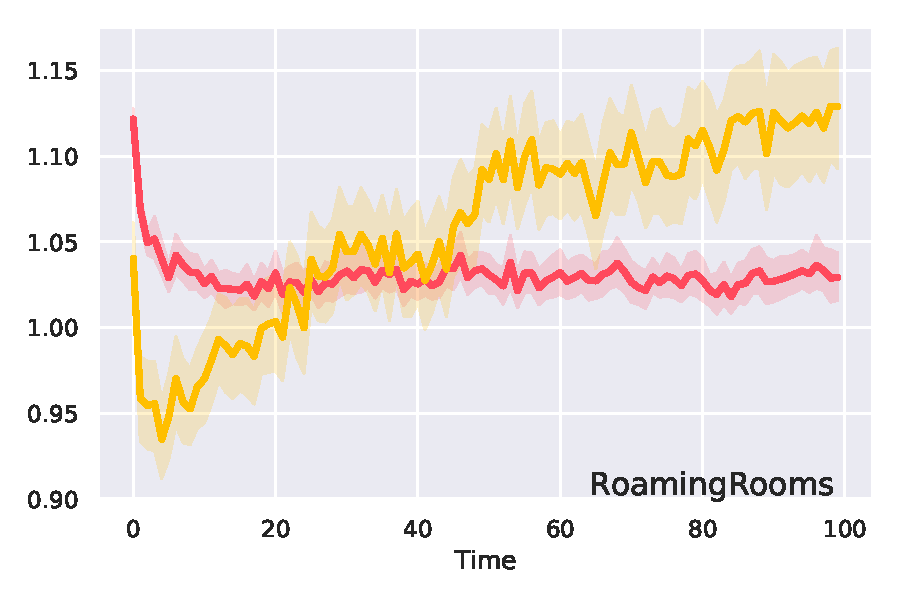
\includegraphics[height=4.0cm,trim={0.3cm 0cm 0cm 0},clip]{figures/matterport-gamma.pdf}
\\
\end{tabular}
\vspace{-0.1in}
\fi
\caption{\textbf{CPM control parameters ($\beta^{r,w}, \gamma^{r,w}$) vs. time.}
\textbf{Left:} \ourchar{} sequences; \textbf{Right:} \ourroom{} sequences; \textbf{Top:}
$\beta^{r,w}$ the threshold parameter; \textbf{Bottom:} $\gamma^{r,w}$ the temperature parameter.}
\label{fig:betagamma}
\end{figure}
